\documentclass[12pt,a4paper]{exam}
\usepackage[latin1]{inputenc}
\usepackage{amsmath}
\usepackage{amsfonts}
\usepackage{amssymb}
\usepackage{makeidx}
\usepackage{graphicx}
\usepackage[left=4.00cm, right=3.00cm, top=3.00cm, bottom=3.00cm]{geometry}
\author{H.O.W.K.E}
\title{Ujian Matematika Tahap II SMP\\, Bangun Ruang, Kesebangunan, dan Kongruensi.\\ OPEN BOOK \\ 120 Menit.}
\begin{document}
	\maketitle
	\paragraph{Bangun Ruang}
	\begin{enumerate}
		\item Berapakah Volume Tabung dengan Luas alas $15\pi cm^2$ dan tinggi 10cm?
		\item Berapakah luas tabung tanpa tutup dengan luas alas $25\pi cm^2$ dan tinggi tabung 7 cm?
		\item Berapakah luas tabung dengan tutup dengan jari-jari alas 6 cm dan tinggi 10 cm?
		\item Berapakah volume kerucut dengan luas alas $30\pi cm^2$ dan tinggi kerucut 3 cm?
		\item Berapakah luas sisi kerucut dengan jari-jari 10 cm, tinggi 24 cm?
		
	\end{enumerate}
	\paragraph{Penyederhanaan Akar}
	\begin{enumerate}
		\item $\sqrt{212}=...\times...=....$
		\item $\sqrt{105}=...\times...=....$
		\item $\sqrt{45}=...\times...=....$
		\item $\sqrt{92}=...\times...=....$ 
		\item 
		$\sqrt{72}=...\times...=....$ 
	\end{enumerate}
	\paragraph{Penyederhanaan Operasi Akar}
	\begin{enumerate}
		\item
		$3\sqrt{17}+5\sqrt{13}-6\sqrt{7}=....$
		\item $4\sqrt{5}+5\sqrt{7}+6\sqrt{7}=....$
		\item $7\sqrt{10}+5\sqrt{10}-6\sqrt{13}=....$ 
		\item $\sqrt{75}+\sqrt{125}+\sqrt{250}=...$
		\item 
		$\sqrt{238}+\sqrt{392}=...$ 
	\end{enumerate}
	\paragraph{Pythagoras}
	\begin{enumerate}
		\item Sebuah $\triangle ABC$ dengan sisi-sisi sebagai berikut yaitu 5 cm, 4cm dan 3cm. Gambarkanlah segitiga tersebut beserta semua sudutnya jika segitiga tersebut siku-siku di $\measuredangle A$!
		\item Terdapat sebuah segitiga siku-siku PQR dengan alas PQ, jika $\measuredangle Q=60\textdegree$ dan hipotenusa $\overline{PQ}=10\sqrt{3}$ cm
		tentukan panjang sisi-sisi lainnya!
		\item Sebuah $\triangle XYZ$ dengan panjang $\overline{XY}$ dan $\overline{XZ}$ adalah 3 cm. Tentukan Luas segitiga tersebut!
		\item Perhatikan gambar berikut!\\
			\includegraphics[scale=0.5]{../Downloads/ma10031}\\
		\\
		Hitunglah nilai a,b,c,d!
		\item Mayang dan Mira naik kapal pesiar dari pelabuhan Tanjung Puting. Keduanya berlayar menuju pulau G dan T seperti pada gambar dibawah ini. Jika Mayang dan Mira dan  berlayar dari pelabuhan pada jam 10.30, dan kecepatan rata-rata Mayang adalah 12 km/jam sedangkan Mira adalah 24 km/jam. Jika pada jam 12.00 mereka berdua sampai di pulau masing-masing secara bersamaan. Berapakah jarak Mira dan Mayang saat itu? 
		\\
		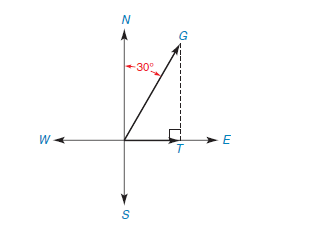
\includegraphics[scale=1]{screenshot002}
		\item Perhatikan gambar berikut!\\
		\includegraphics[width=0.7\linewidth]{../Downloads/ma10032}
		\\
		Hitunglah nilai e,f,g!


	\end{enumerate} 
		\paragraph{Kesebangunan dan Kongruensi}
		\begin{enumerate}
			\item Perhatikan Gambar berikut!\\
			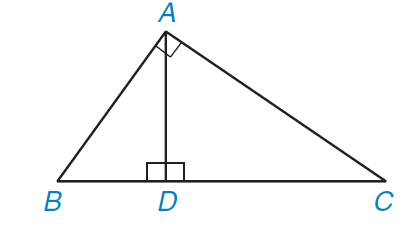
\includegraphics[width=0.5\linewidth]{screenshot003}
			
			Diketahui : $\overline{BD}=10$ cm, $\overline{CD}=16$ cm.
			\\
			Ditanyakan :
				\begin{enumerate}
					\item panjang $\overline{AD}$?
					\item panjang $\overline{AB}$?
					\item panjang $\overline{AC}$?
					\item panjang $\overline{BC}$?
					\item luas $\triangle{ABC}$?
					\item luas $\triangle{ADB}$?
					\item luas $\triangle{ABC}$?
				\end{enumerate}
				\item Perhatikan Gambar dibawah ini!\\
				\includegraphics[width=0.5\linewidth]{../Downloads/kesebangunan-trapesium}\\
				Jika trapesium $PQTU$ $\cong$ trapesium $TUSR$ berapakah panjang $\overline{TU}$ dan $\overline{SR}$?
				\item Sebuah foto berukuran tinggi 30 cm dan lebar 20 cm ditempel pada sebuah karton. Sisa karton di sebelah kiri, kanan, atas foto 2 cm. Jika foto dan karton sebangun, sisa karton di bawah foto adalah?
				\item Berapakah x pada gambar dibawah ini?
				\begin{center}
				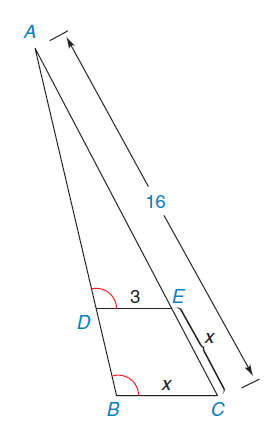
\includegraphics[scale=0.4]{screenshot004}\end{center}
			
				\item Perhatikan gambar berikut!
				
				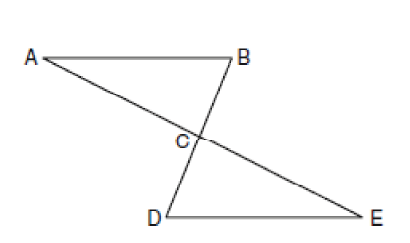
\includegraphics[scale=0.5]{screenshot005}
				
				jika $\overline{BD}$ membelah $\overline{AE}$ sama rata dan $\overline{AE}$ membelah $\overline{BD}$ sama rata , buktikanlah jika $\triangle ABC \cong \triangle CDE$!




		\end{enumerate}	
	
\end{document}